\begin{figure}[htbp]
  \centering
  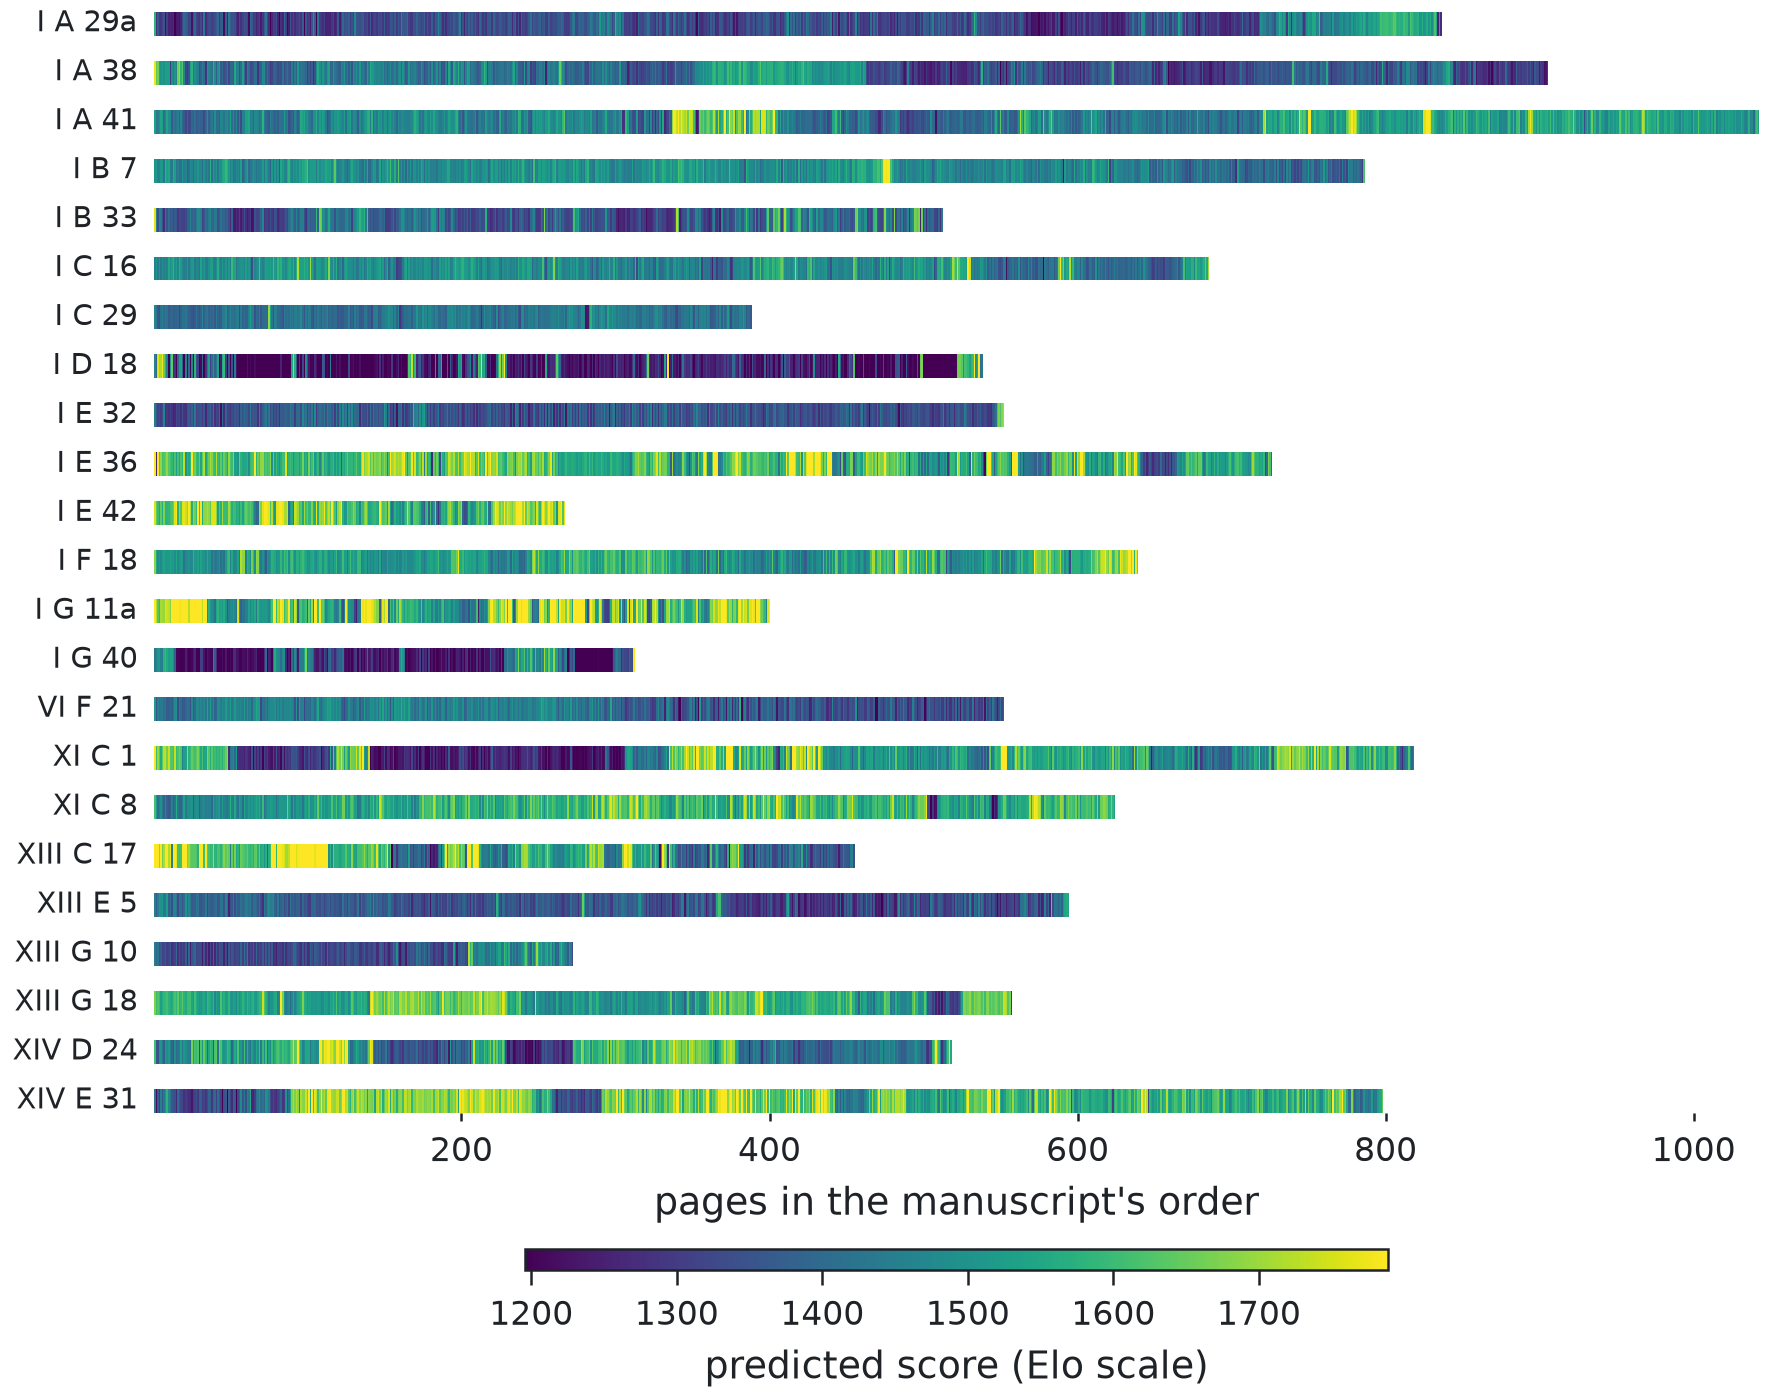
\includegraphics[width=15.00cm]{figures/manuscript_strips.png}
  \caption{The 23 manuscripts' leaf pages, one row each in the catalogue's order, each page a band coloured by its predicted score, in the manuscript's order from the left; the rows' lengths are the manuscripts' numbers of leaf pages. A page's predicted score is its expected Elo score: the regression of the dataset's Elo scores on the ensemble's out-of-fold scores, 1,500 + 168 $\times$ $z$, $z$ being the page's score under the ensemble of the Layout (geometry) and ViT rankers (equal weights). The rankers were trained without the dataset's pages from XIII G 10, I E 36, I A 29a and I A 38, so every score is out of sample. The 362 leaves on which Kraken finds fewer than 5 text lines (blank or nearly blank) are left out. Catalogue facts from Dragoun, Ebersonová and Doležalová (2021).}
  \label{fig:manuscript_strips}
\end{figure}
